\documentclass[11pt]{article}
\title{Machine Learning Homework 02 – Report}
\author{Adam Catto}
\date{ }
\usepackage{graphicx}

\usepackage{amsmath}
\newcommand{\y}{\mathbf{y}}
\begin{document}
\maketitle
\section{Introduction}
The main goal of this assignment is to implement a linear classifier to perform multiclass classification. In order to initialize the relevant weights $\omega$ for the classifier, there are two approaches to take: 
\begin{enumerate}
	\item Initialize $\omega$ with the first data point of the dataset
	\item Initialize $\omega$ using linear regression
\end{enumerate}
For approach (2), we are meant to also implement our own linear regression algorithm. Finally, we are to train and validate our implementation using 5 samples from the scikit-learn datasets ``Breast cancer'' and ``Iris''.

\section{Solution}

\subsection{Linear Regression Implementation}
To do linear regression, we are to solve the least squares error problem for a dataset. We have a system of equations represented as 
$$ X\omega = \mathbf{y}$$We can approximate a solution to this by setting a residual error term $r = \mathbf{y} - X\omega $, and minimize the size of $r$ – this is called the least-squares approximate solution of a system of equations.\\ 
 \\
To compute this minimization, we take the following steps:
\begin{gather}
	\min ||r||\\ 
	\min ||(\mathbf{y} - X\omega)|| \\
	\min (\mathbf{y} - X\omega)^T (\mathbf{y} - X\omega) \\
	\min \mathbf{y}^T\mathbf{y} - \mathbf{y}^T X\omega - \omega^T X^T \mathbf{y} + 
	\omega^T X^T X \omega  \\
		\nabla _{\omega} \left( \mathbf{y}^T\mathbf{y} - \mathbf{y}^T X\omega - \omega^T X^T \mathbf{y} + 	\omega^T X^T X \omega  \right) = 0\\
		- \y^T X + \omega^T X^T X = 0\\
		\omega^T X^T X = \y^T X		\\
		X^T X \omega = X^T \y \\
		\omega = ((X^T X)^{-1}X^T)\y
\end{gather}
This is precisely the Moore-Penrose pseudoinverse of $X$ multiplied by $\y$. It is in this way that we solve the least squares approximation problem for linear regression, in a compact and vectorized manner.

\subsection{Linear Classifier Implementation}
I implemented a multiclass perceptron classifier. The first step is to initialize the weight vector of a linear model for each class in the dataset – this can be done in a number of ways, two of which are implemented in this project: (1) initialization by linear regression on the training data, (2) initialization using the first data point in the dataset. Next, iterate over the dataset and predict the label by taking the $argmax$ of the product of the weight vector and the current feature vector (represented as a row in the feature matrix $X$) over all linear models (linear functions associated with each label) – if the prediction is correct, then proceed to the next data point; if not, then update the linear model of both the target label and the predicted label by the difference between weights and the feature vector, times an optional learning rate. This is the gradient descent method. \\ 
 \\
What is happening here is that we are building decision boundaries based on the line-of-best-fit; the magnitude of the y-value predicted by each function is proportional to the model's confidence that the feature vector is in the associated class. When updating the linear models for the target and predicted classes, we are moving the decision boundary of each to accommodate the observed classification error.

\section{Training and Validation}
\subsection{Experiment}
The classifier was profiled on the iris and breast cancer datasets found in sklearn.datasets. Iris has 3 classes, 4 features, 150 samples, and Breast cancer has 2 classes, 30 features, 569 samples. Each dataset was sampled 5 times, using an 80/20 train/test split percentage. This was done for both initialization methods: linear regression and first-value initialization. The weight improvement method was done over a fixed number of iterations (10,000), with a learning rate of 0.01. The errors were evaluated at the end of each iteration (epoch), and plotted as a function of the iteration.

\subsection{Results}
The classifier performed similarly on both datasets, and using both initialization methods, with the iris dataset achieving slightly better results than the breast cancer dataset. It achieved an average accuracy of about 95\% for the iris dataset and an an average accuracy of about 87\% for the breast cancer dataset. Using the linear regression initialization method, the classifier on average scored 91.6\% accuracy on the breast cancer dataset  and 94\% accuracy on the iris dataset. Using the first-value initialization method, the classifier on average scored 88.8\% accuracy on the breast cancer dataset and 96\% accuracy on the iris dataset. We can observe their performance more visually across the five samples using these two plots:\\
$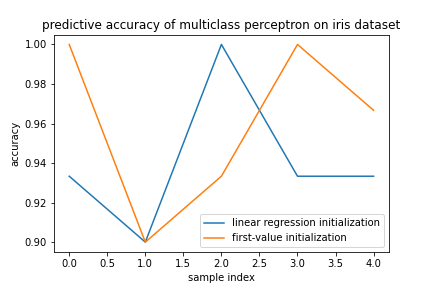
\includegraphics[scale=0.41]{../src/iris_accuracies.png} 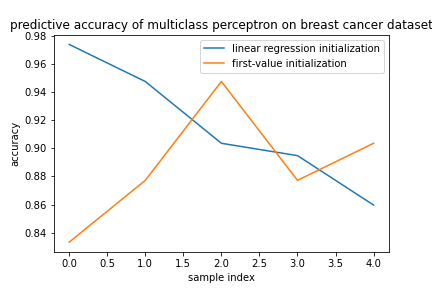
\includegraphics[scale=0.41]{../src/bc_accuracies.png}$

The weight updating converged to somewhere between 86\% and 96\% for both initialization methods very quickly, as we can see from the following plots:\\
$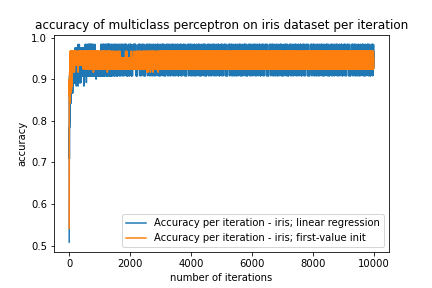
\includegraphics[scale=0.41]{../src/iris_errors.png} 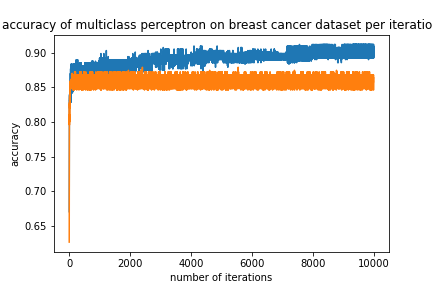
\includegraphics[scale=0.41]{../src/bc_errors.png}$\\


\subsection{Discussion}
The similar performance across initialization methods was to be expected. The algorithm adjusts the weights quickly, and over so many iterations the training algorithm catches up. Still, the linear regression initialization seems to provide slightly better results; this can be explained due to the fact that the weights begin at a more ideal value than in first-value initialization, since the regression allowed for learning from all other present data. The small advantage seems to stay with the regression initialization, as the first-value initialization error per iteration is always slightly larger. \\
 \\
It is also interesting that the iris dataset yields better accuracy, since it has much fewer samples than the breast cancer dataset, and more classes. Perhaps this is explained by the fact that the breast cancer dataset has many more features than the iris dataset, which may lead the model to overfit more often on the breast cancer dataset than on the iris dataset. Indeed, this appears to happen as we can see from the accuracy per iteration plots: there is slightly more error (less correct classifications) on the breast cancer dataset than there is on the iris dataset. This appears to be an explanatory factor in the outperformance of the classifier on iris vs. breast cancer.\\
 \\
What we have seen from this study is that there are several critical factors that affect the performance of a linear classifier. These appear to be the number of samples (more examples yields more learning opportunities) and the number of features (more features may lead to overfitting).
\end{document}